\documentclass[12pt,a4paper]{article}
\usepackage[utf8]{inputenc}[spanish]
\usepackage{amsmath}
\usepackage{amsfonts}
\usepackage{amssymb}
\usepackage{lmodern}
\usepackage{amsmath}
\usepackage{amsthm}
\usepackage{enumerate}
\usepackage{graphicx}
\usepackage{mathtools}
\usepackage{stackrel}
\usepackage{multicol}
\usepackage[left=2cm,right=2cm,top=2cm,bottom=2cm]{geometry}
\newcounter{neq}
\providecommand{\abs}[1]{\lvert#1\rvert}
\newcommand{\SIGMA}{\Sigma^{\ast}}
\newcommand{\N}{\noindent}

\title{Resumen Física}

\begin{document}
	\begin{center}
		\Huge \textbf{Resumen Física para Computación FaMAF 2017 - P3: Termodinámica}  \\
		\vspace{3mm}
		\large Agustín Curto
	\end{center}

	\section{Temperature}
		\N 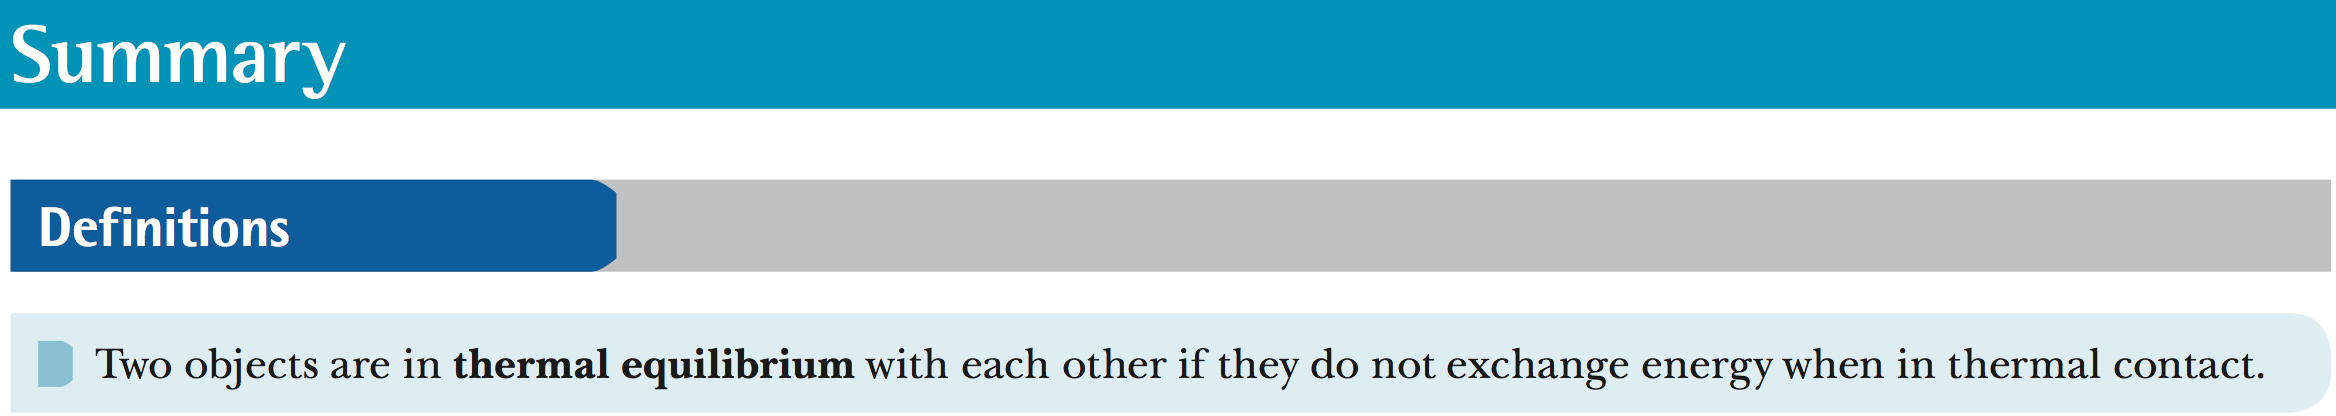
\includegraphics[scale=.42]{1_a.png}
		
		\vspace{2mm}
		\N 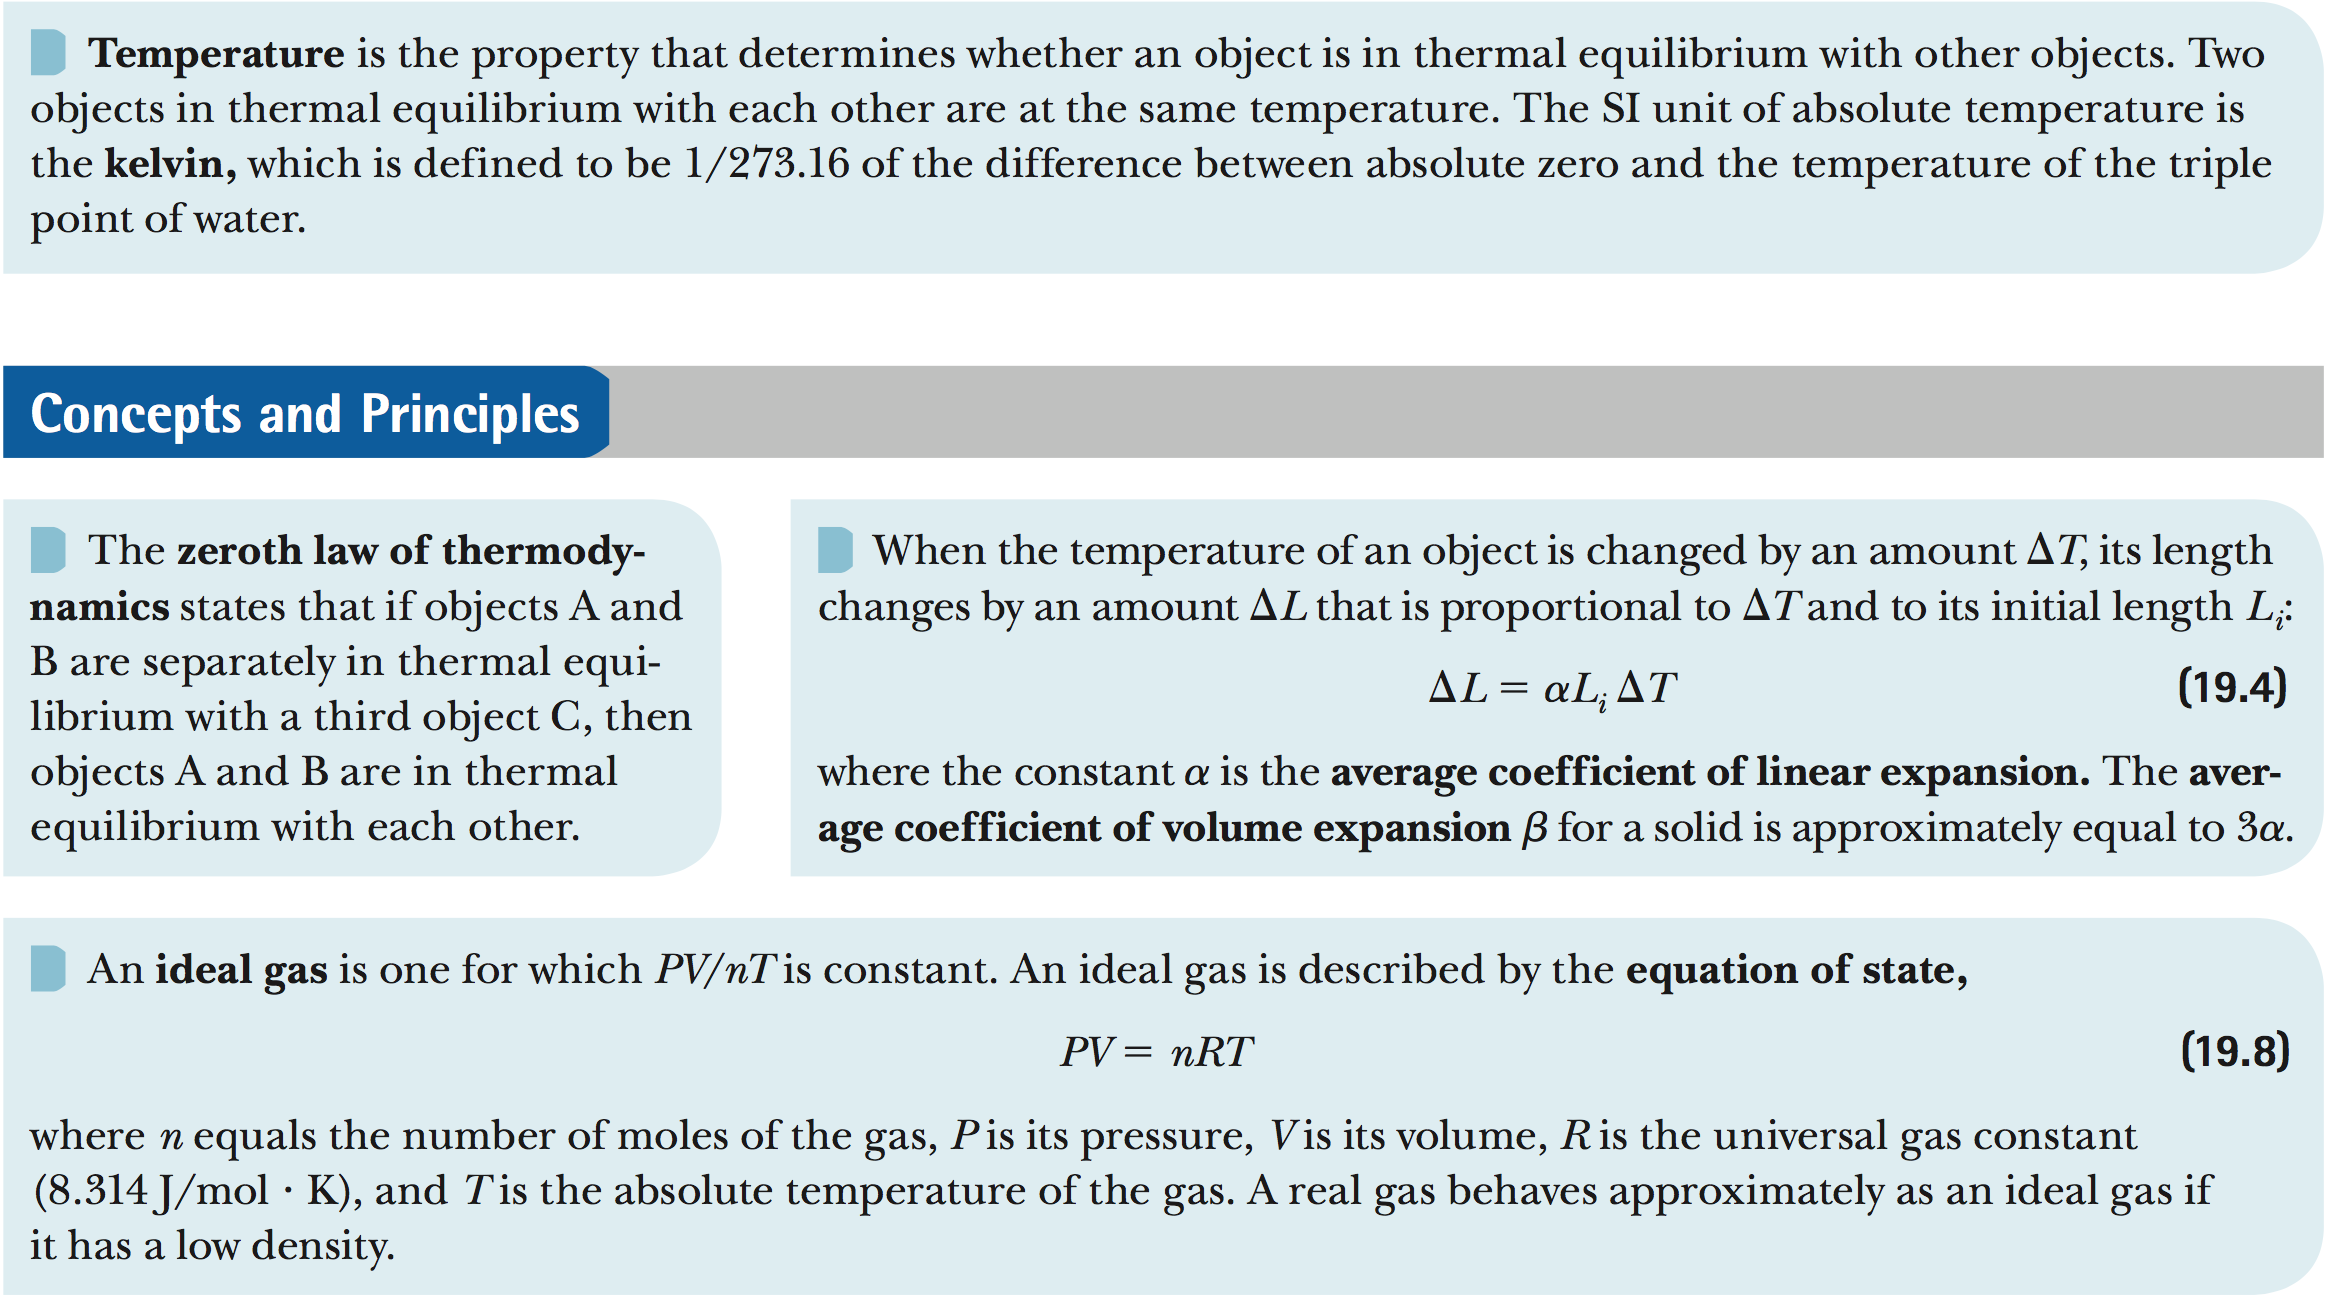
\includegraphics[scale=.42]{1_b.png}
		
	\section{The first law of thermodynamics}
		\N 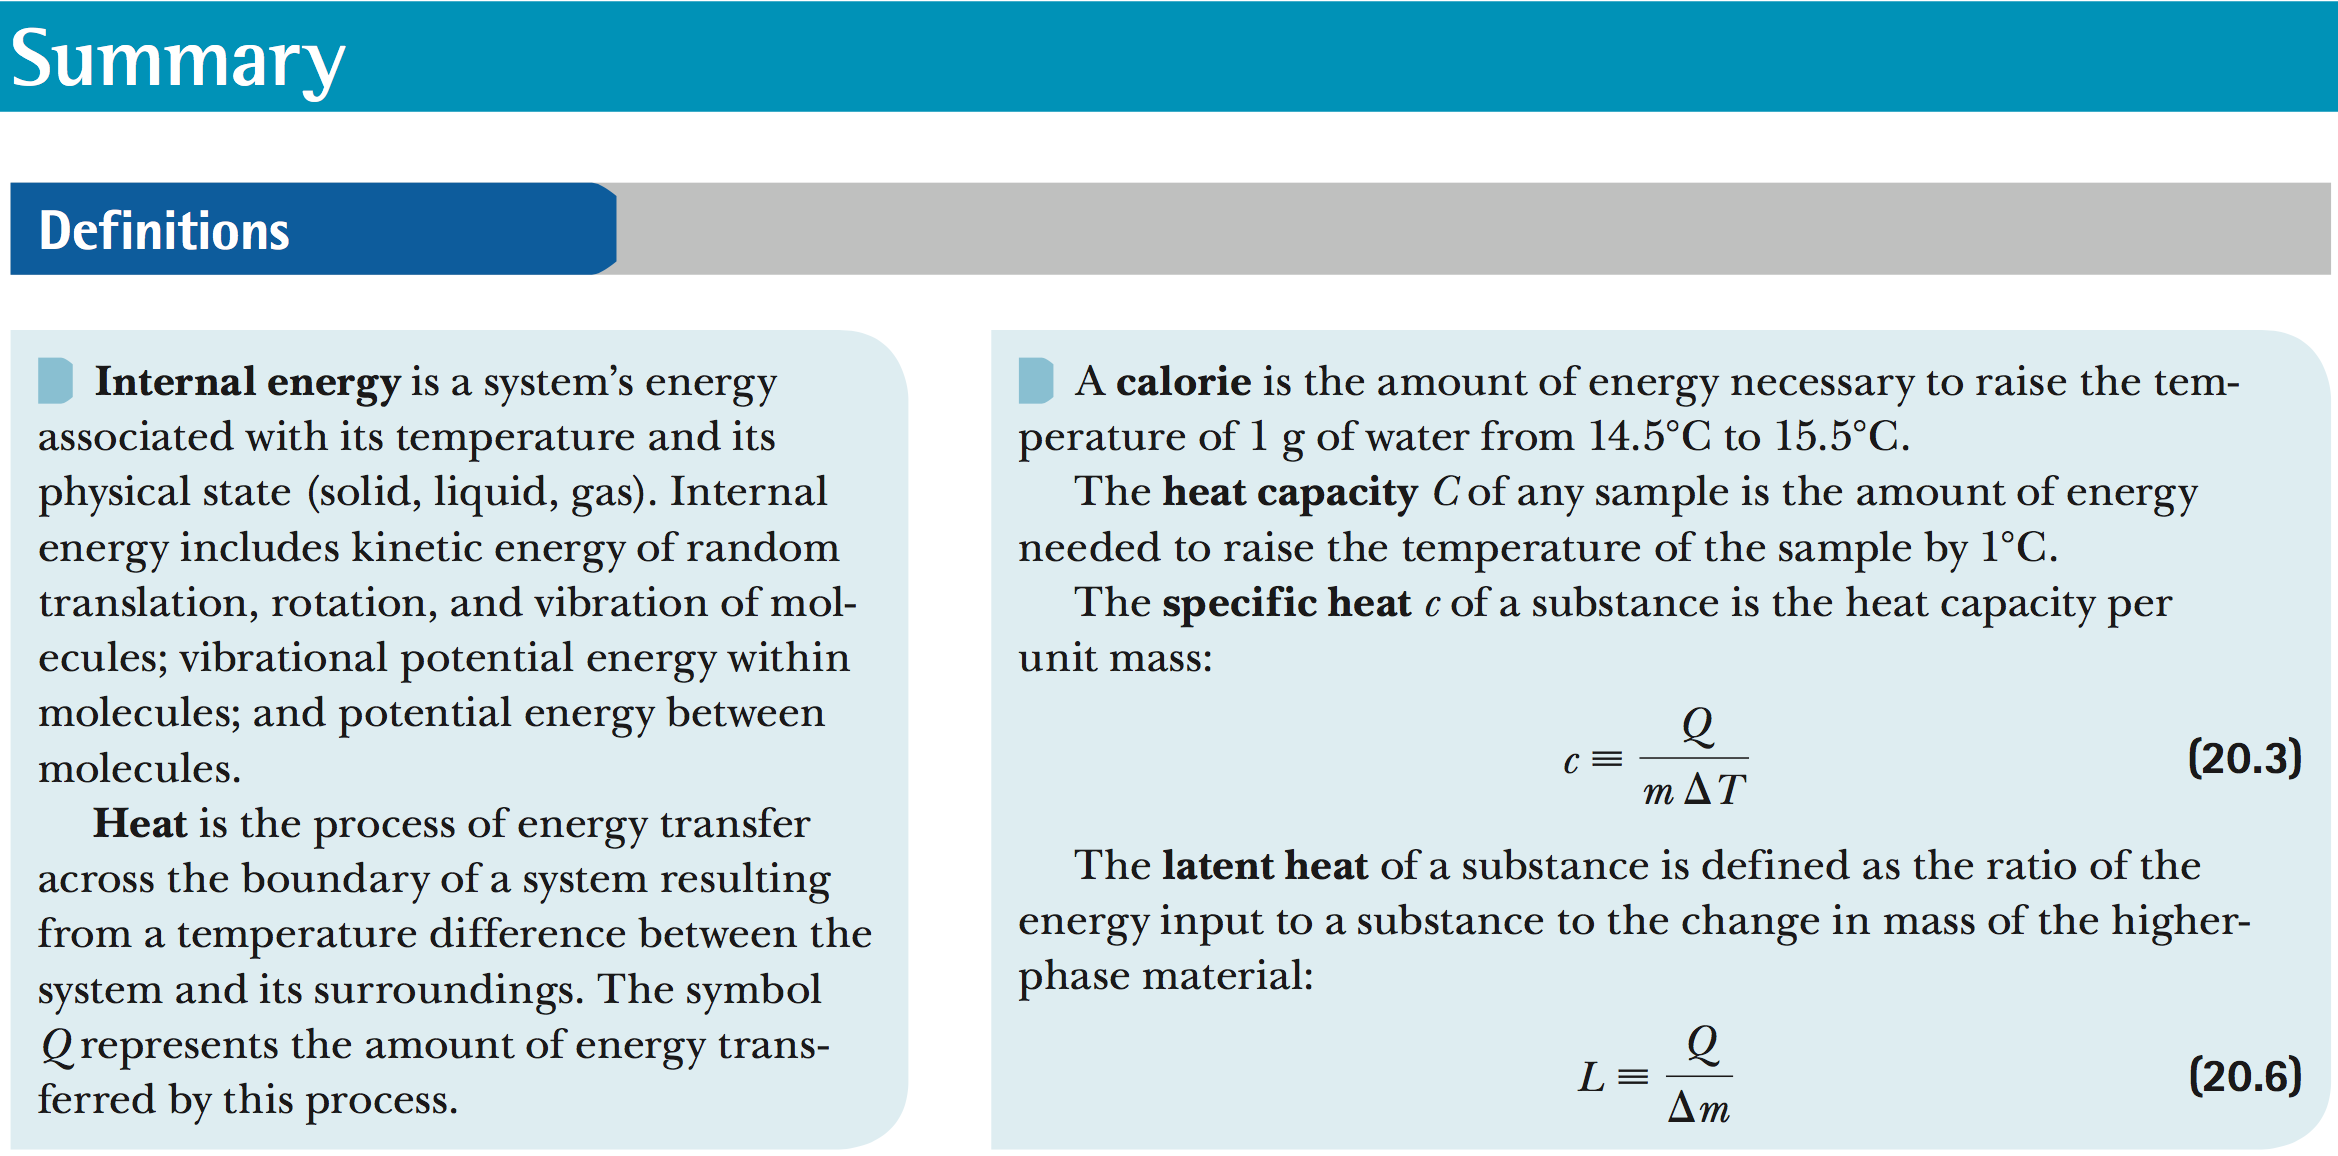
\includegraphics[scale=.42]{2_a.png}
		
		\vspace{2mm}
		\N 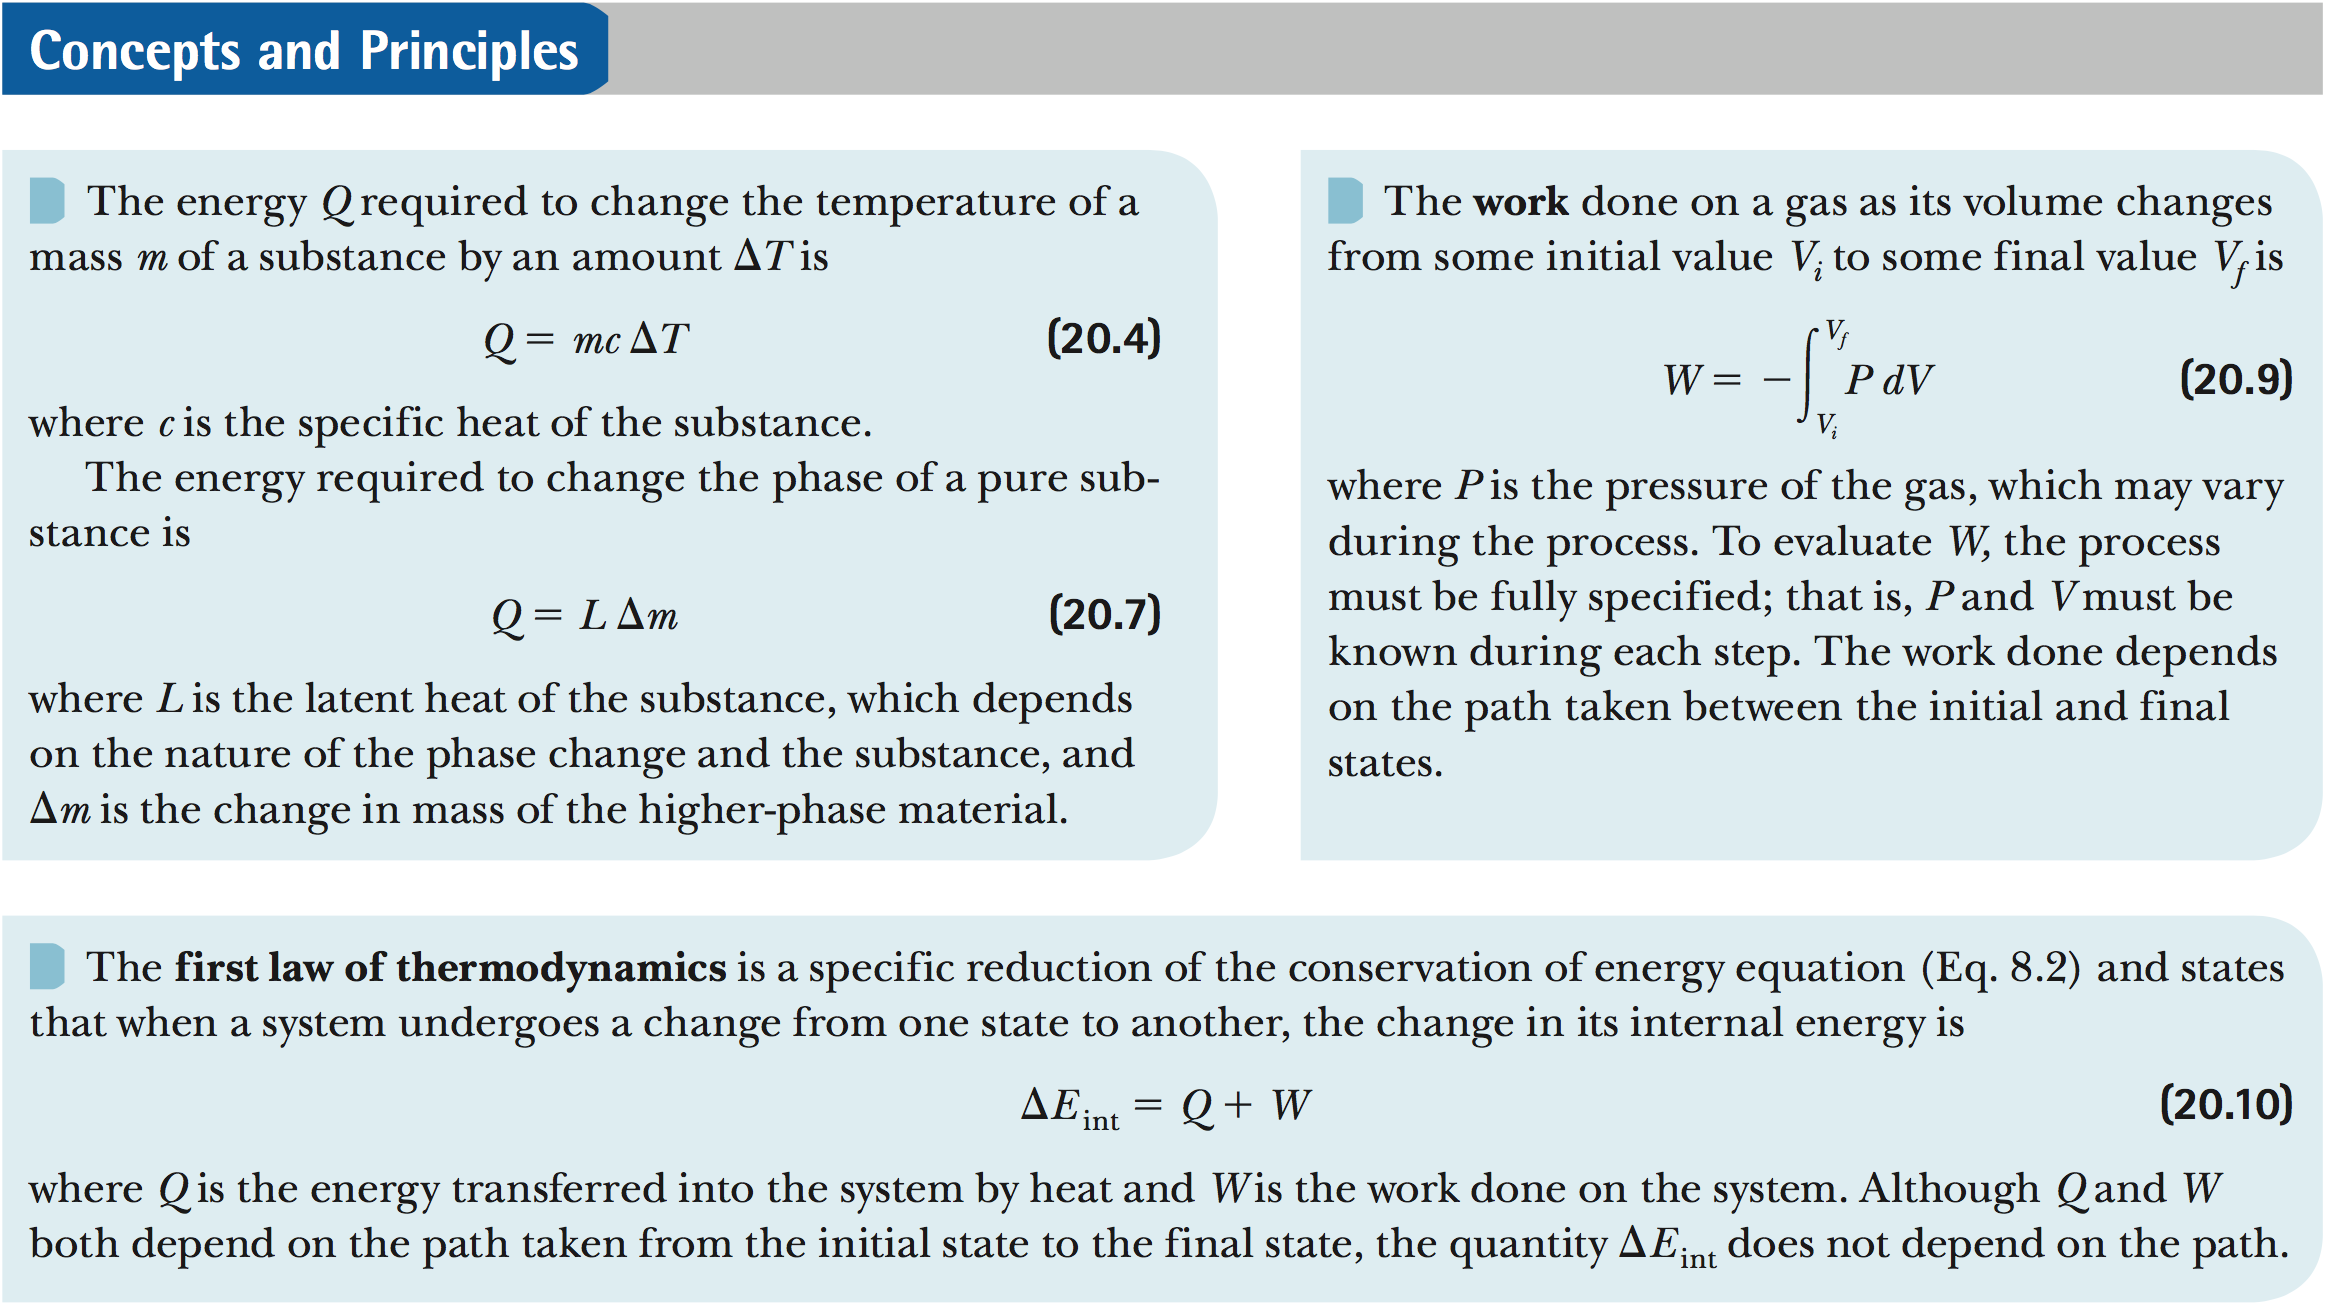
\includegraphics[scale=.42]{2_b.png}
		
		\vspace{2mm}
		\N 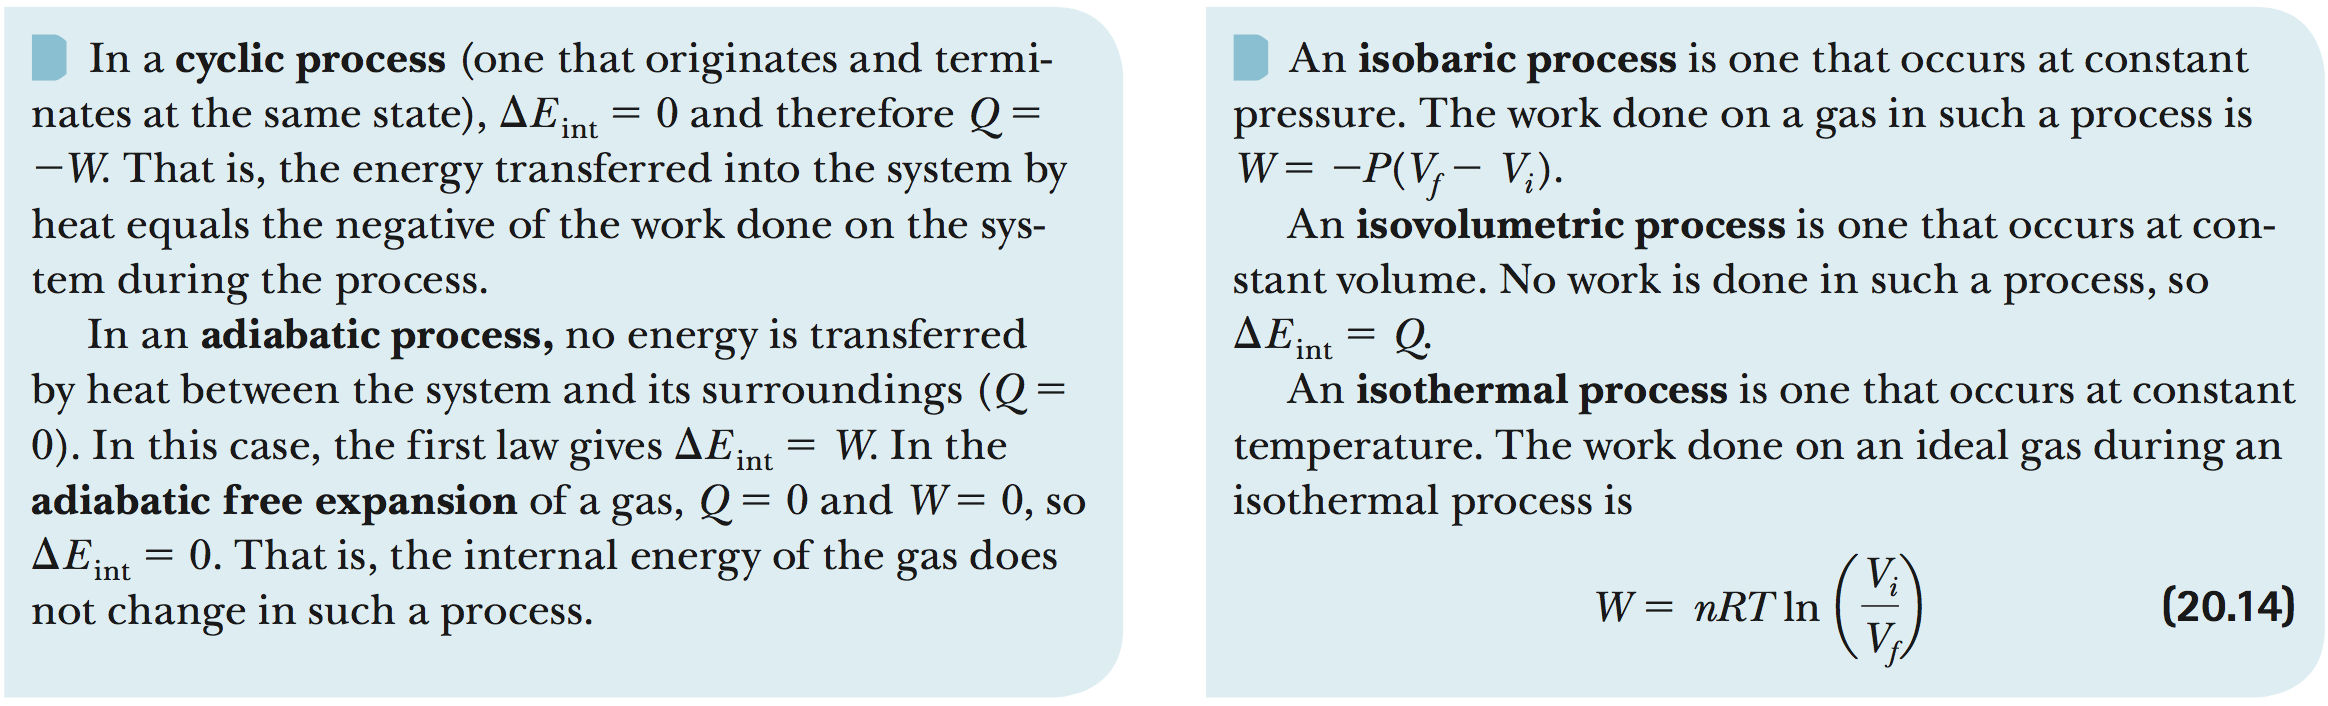
\includegraphics[scale=.42]{2_c.png}
		
		\vspace{2mm}
		\N 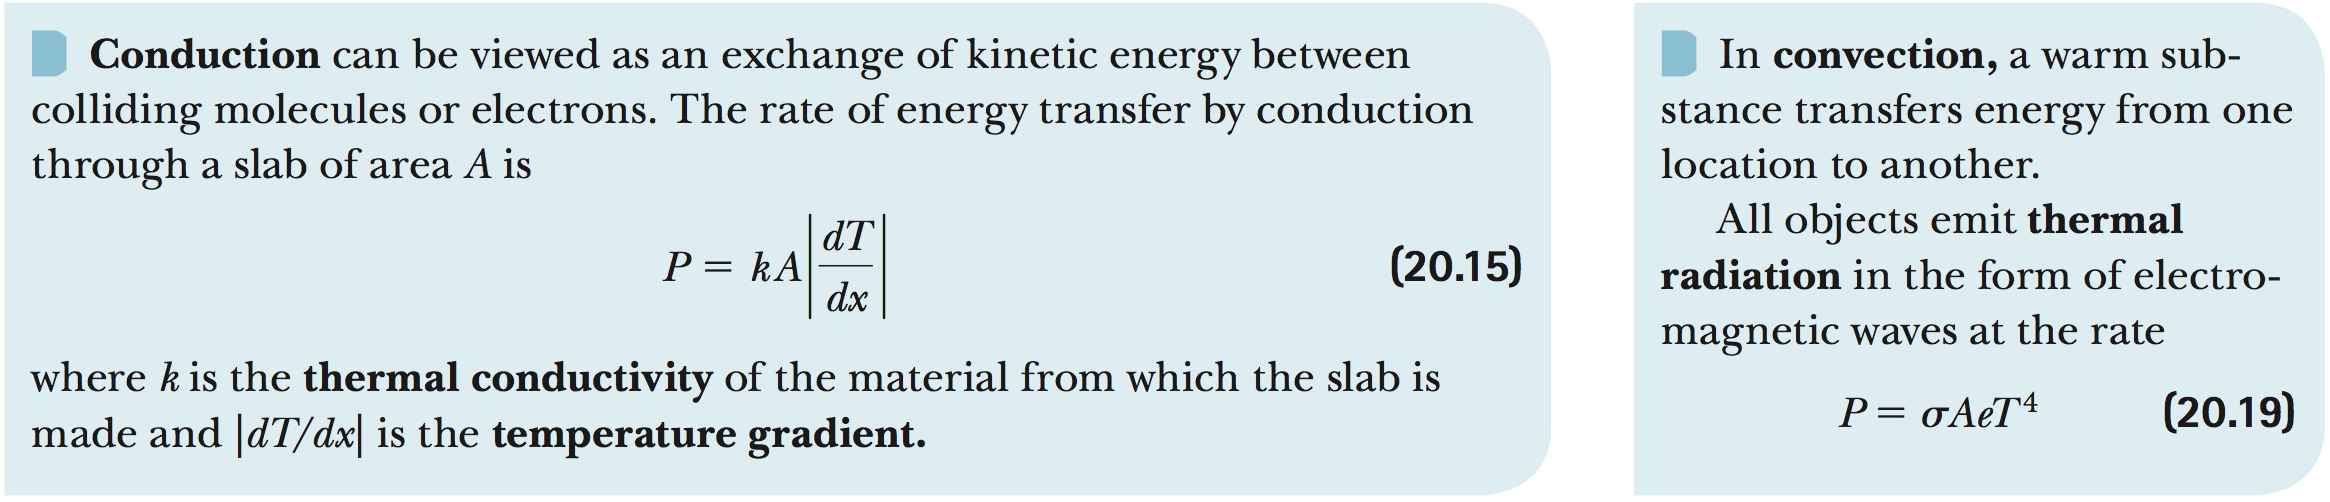
\includegraphics[scale=.42]{2_d.png}
		
	\section{The kinetic theory of gases}
		\N 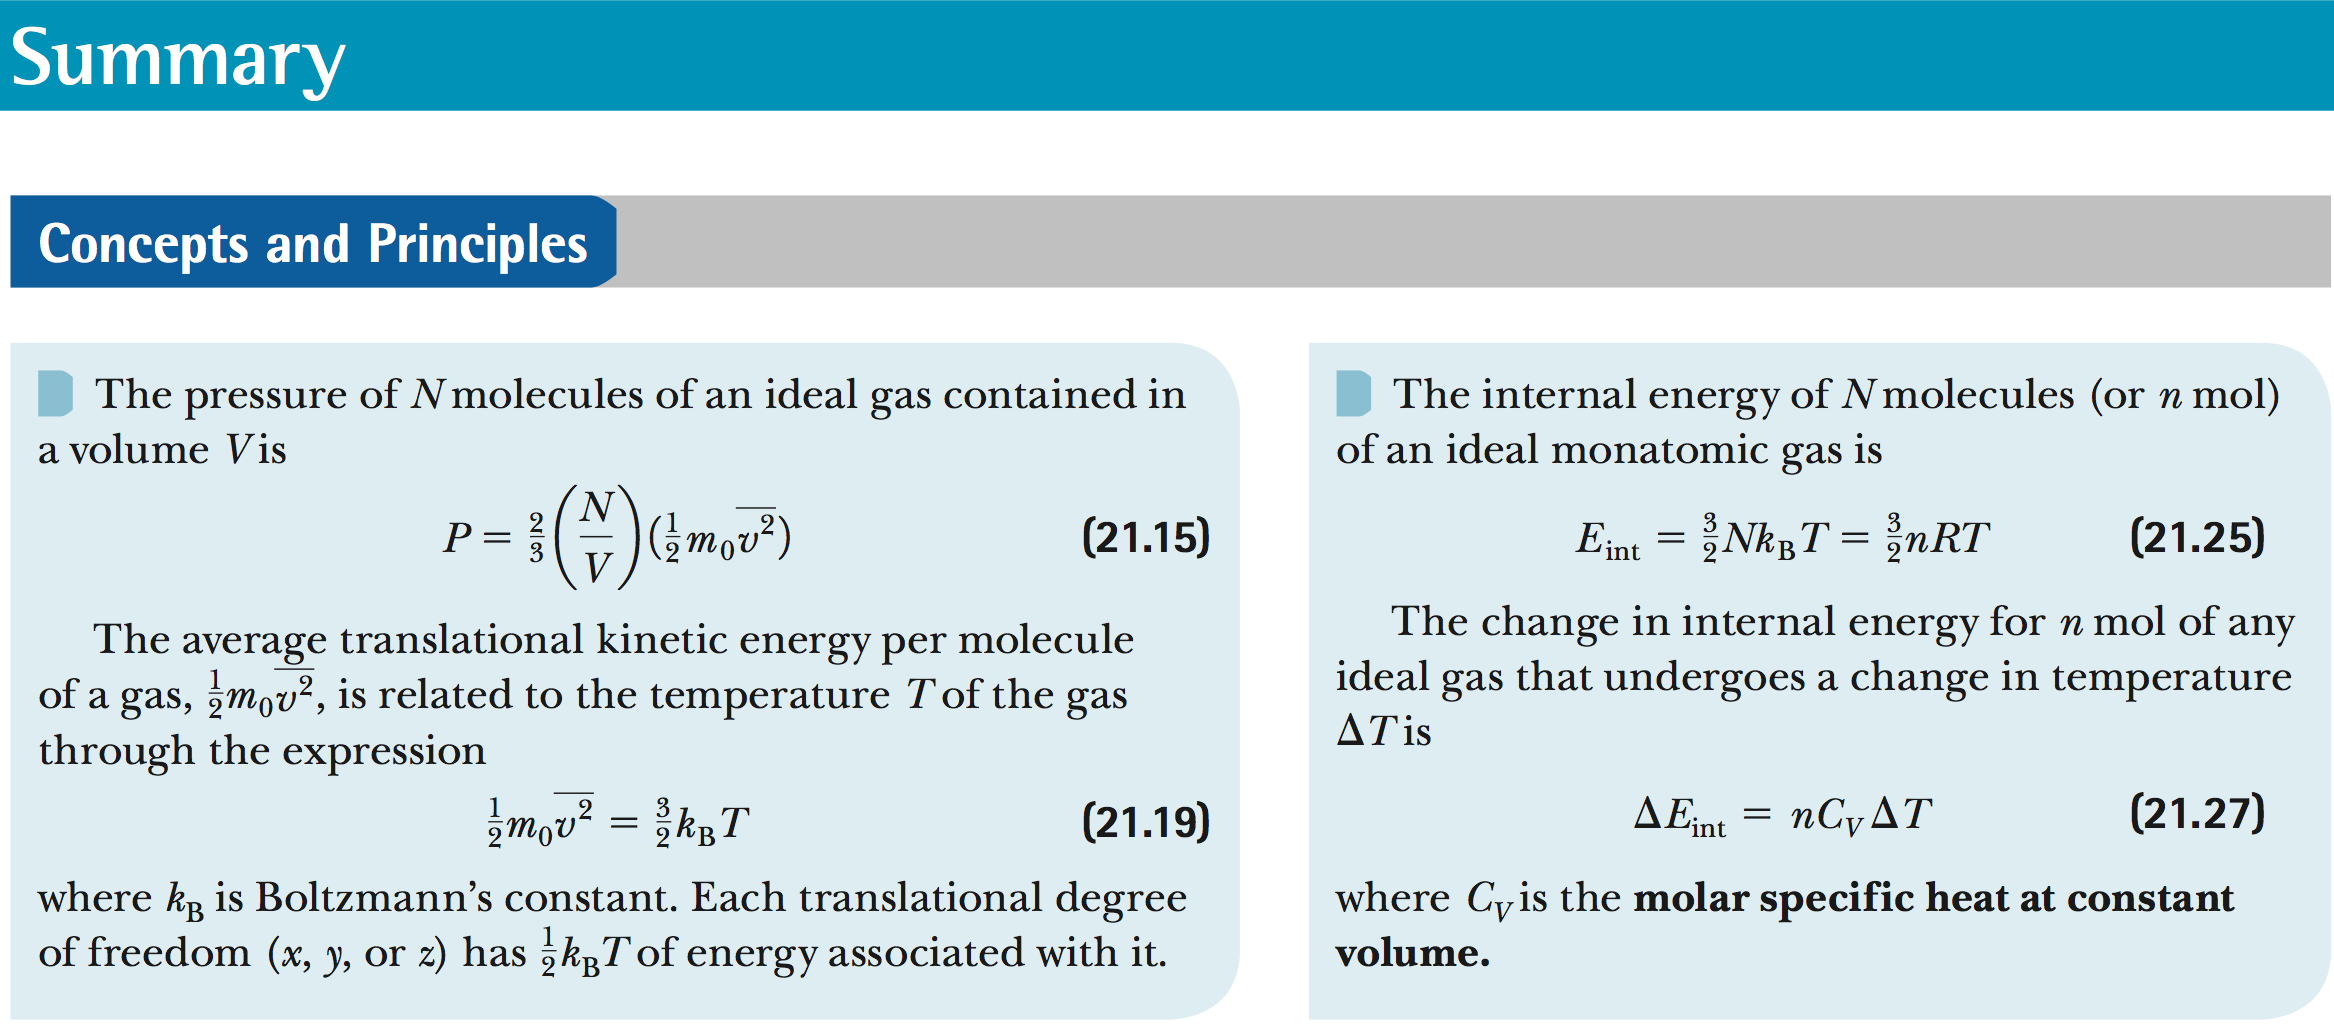
\includegraphics[scale=.42]{3_a.png}
		
		\vspace{2mm}
		\N 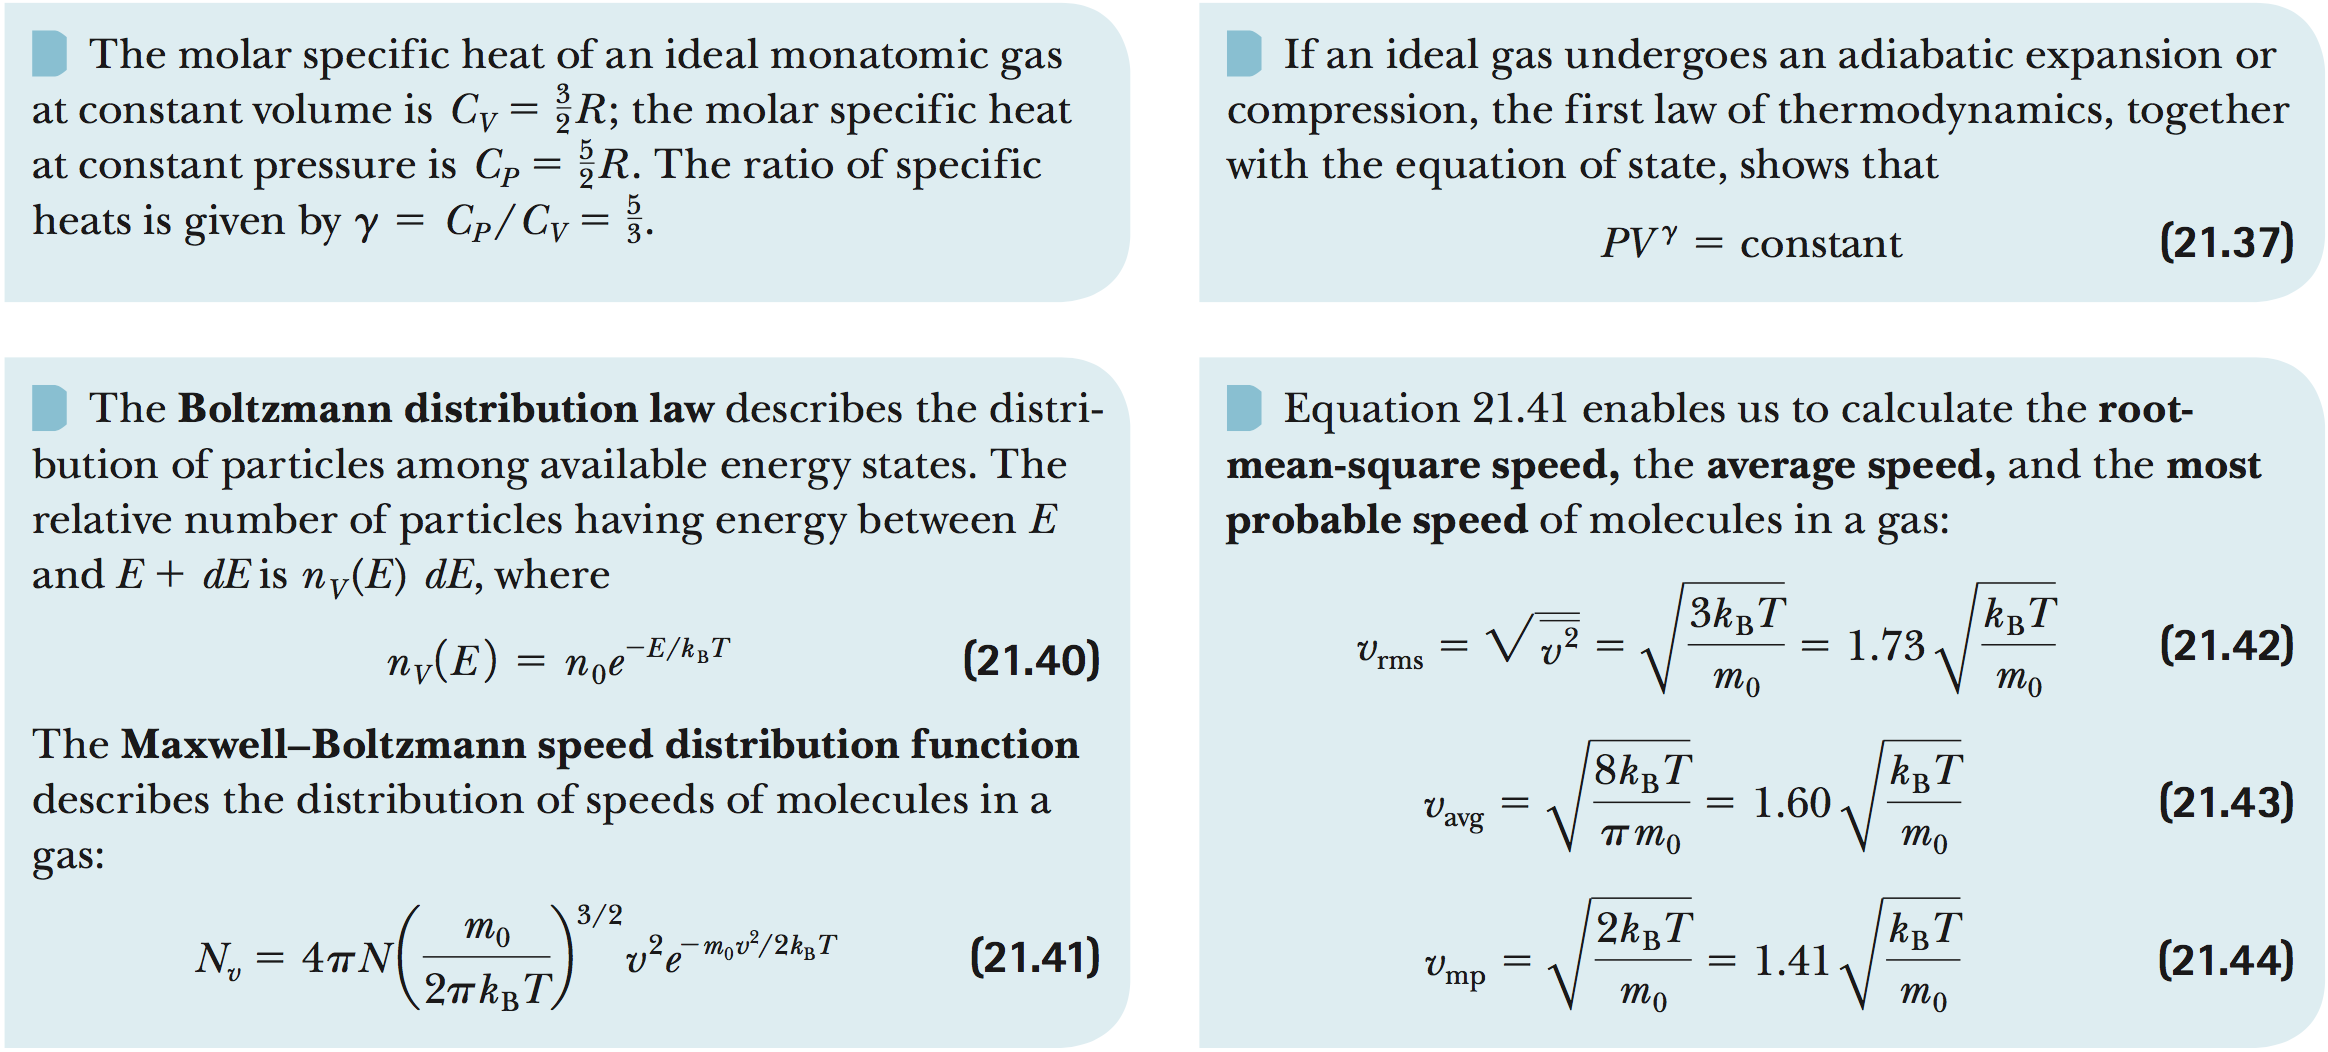
\includegraphics[scale=.42]{3_b.png}
		
	\section{Heat engines, entropy, and the second law of thermodynamics}
		\N 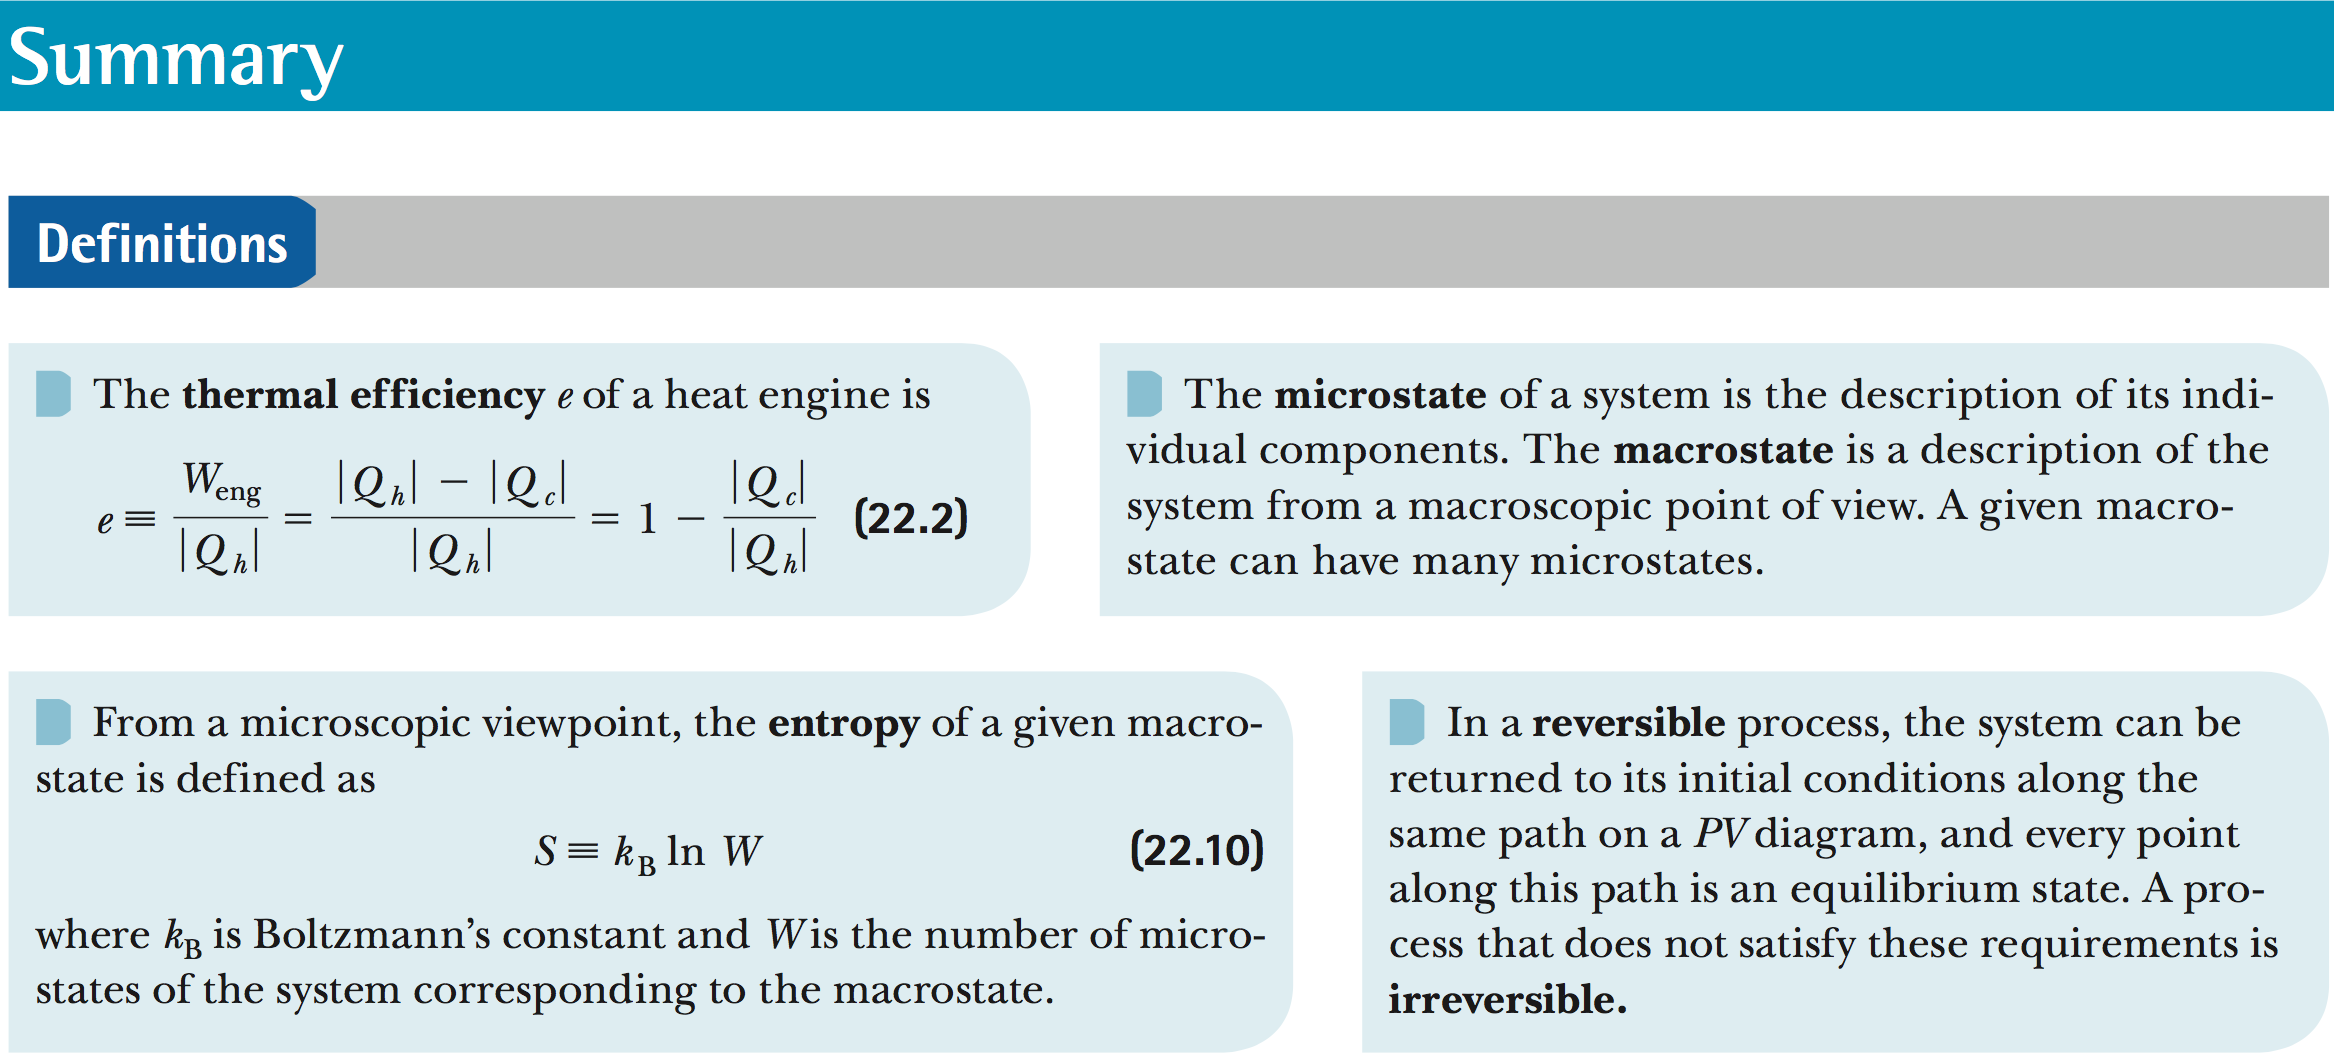
\includegraphics[scale=.42]{4_a.png}
		
		\vspace{2mm}
		\N 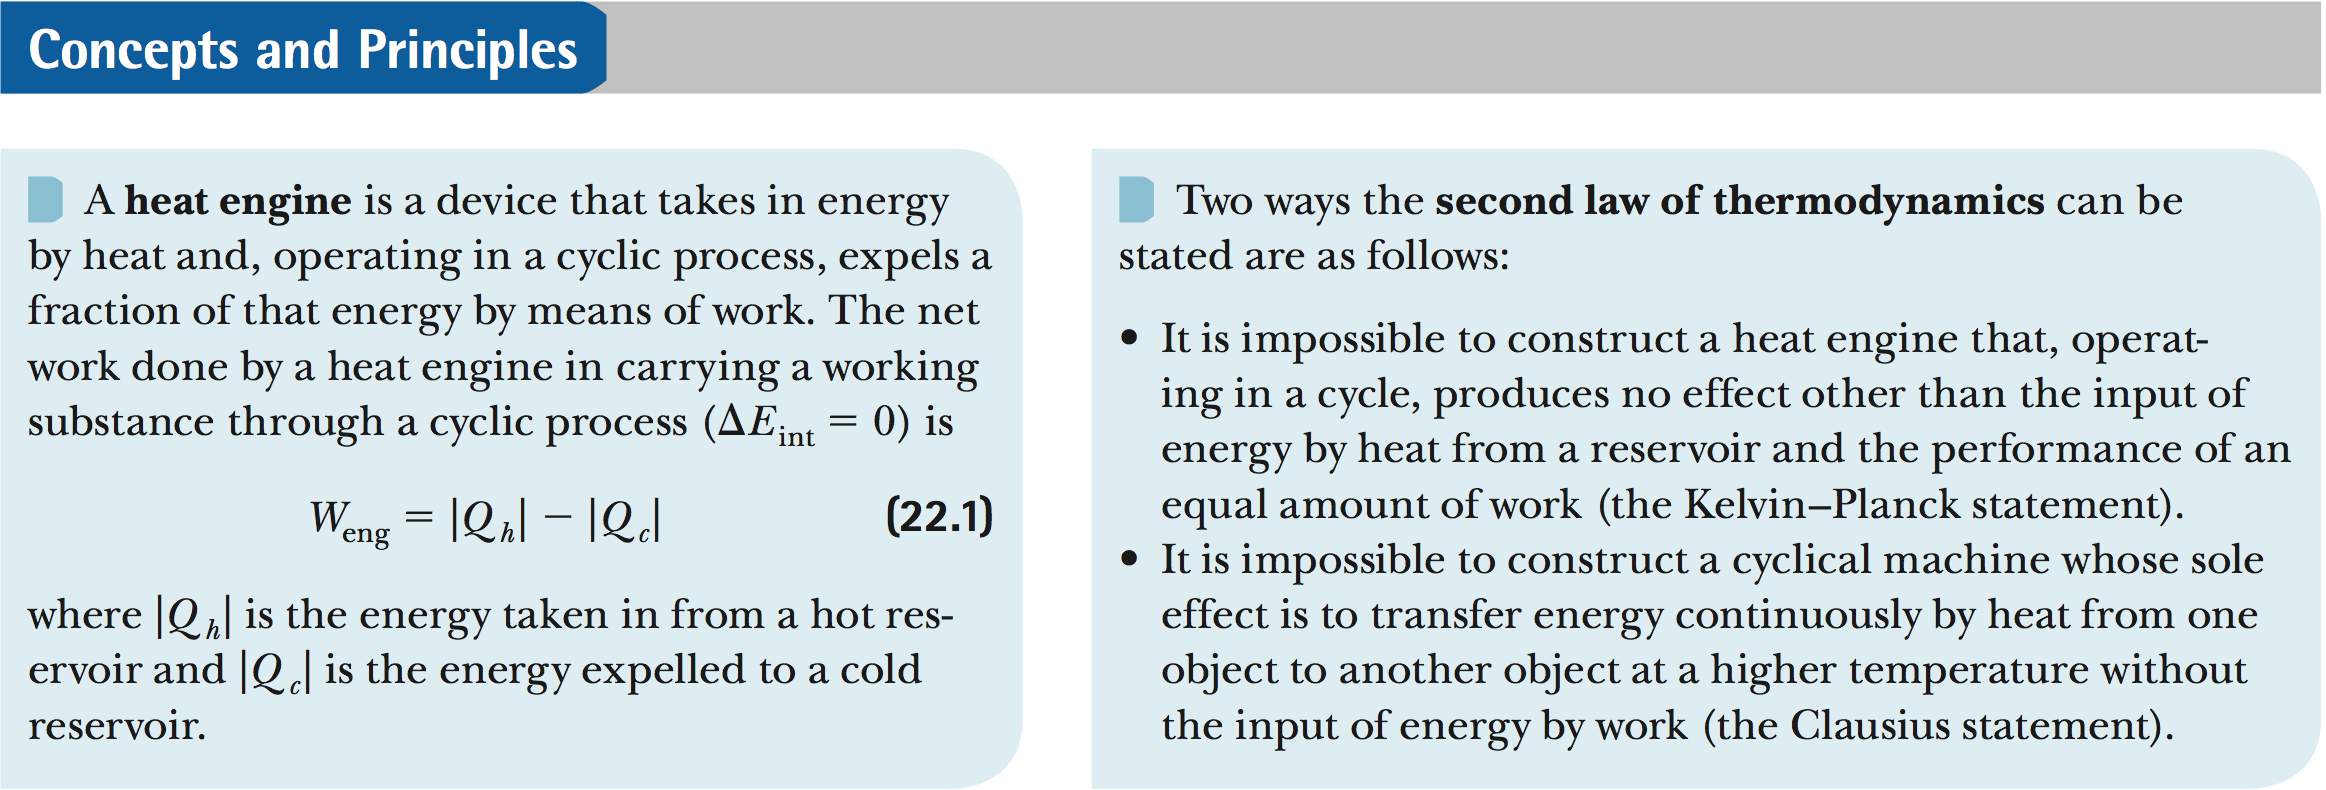
\includegraphics[scale=.42]{4_b.png}
		
		\vspace{2mm}
		\N 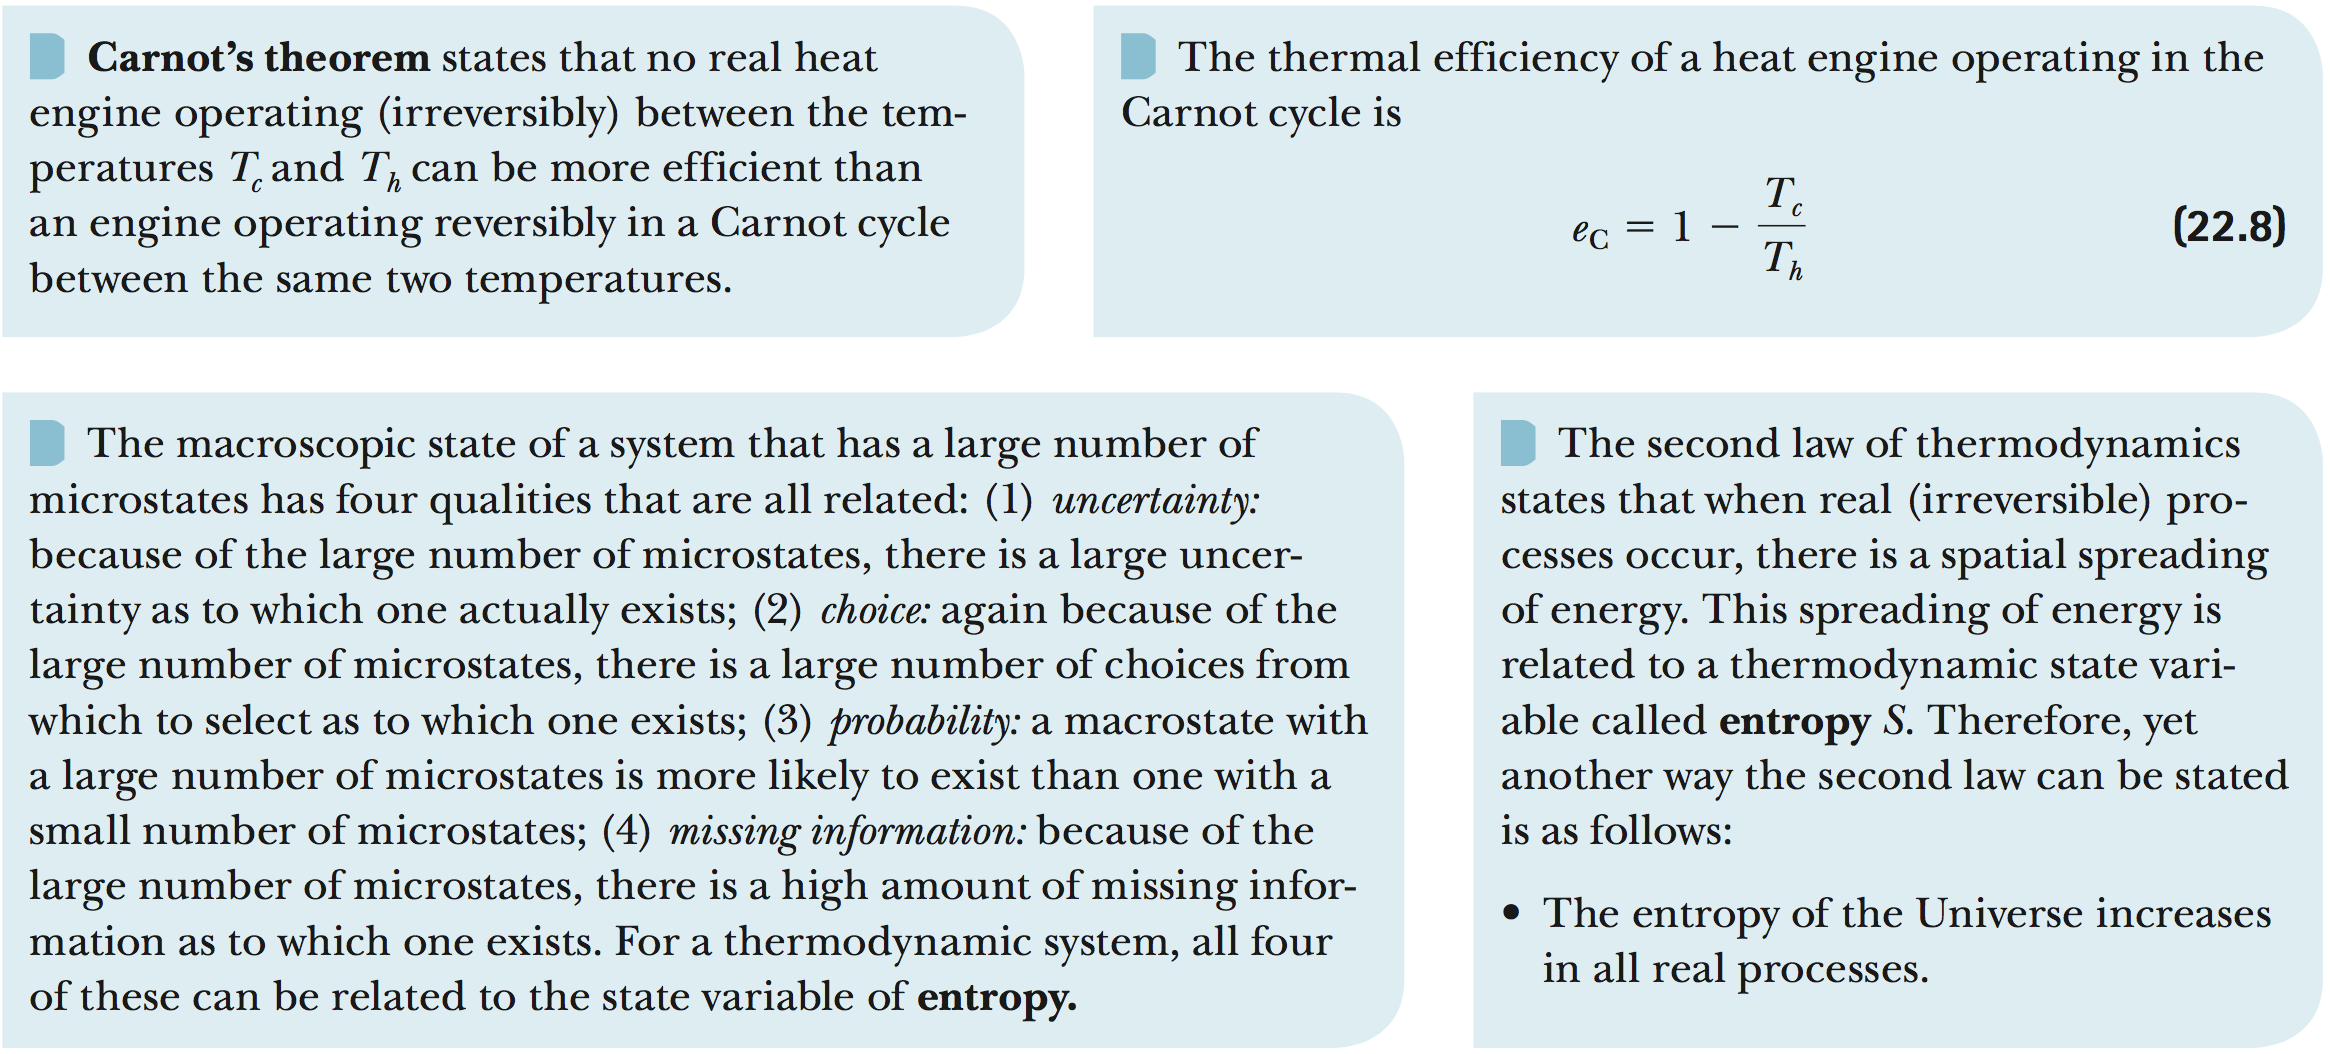
\includegraphics[scale=.42]{4_c.png}
		
		\vspace{2mm}
		\N 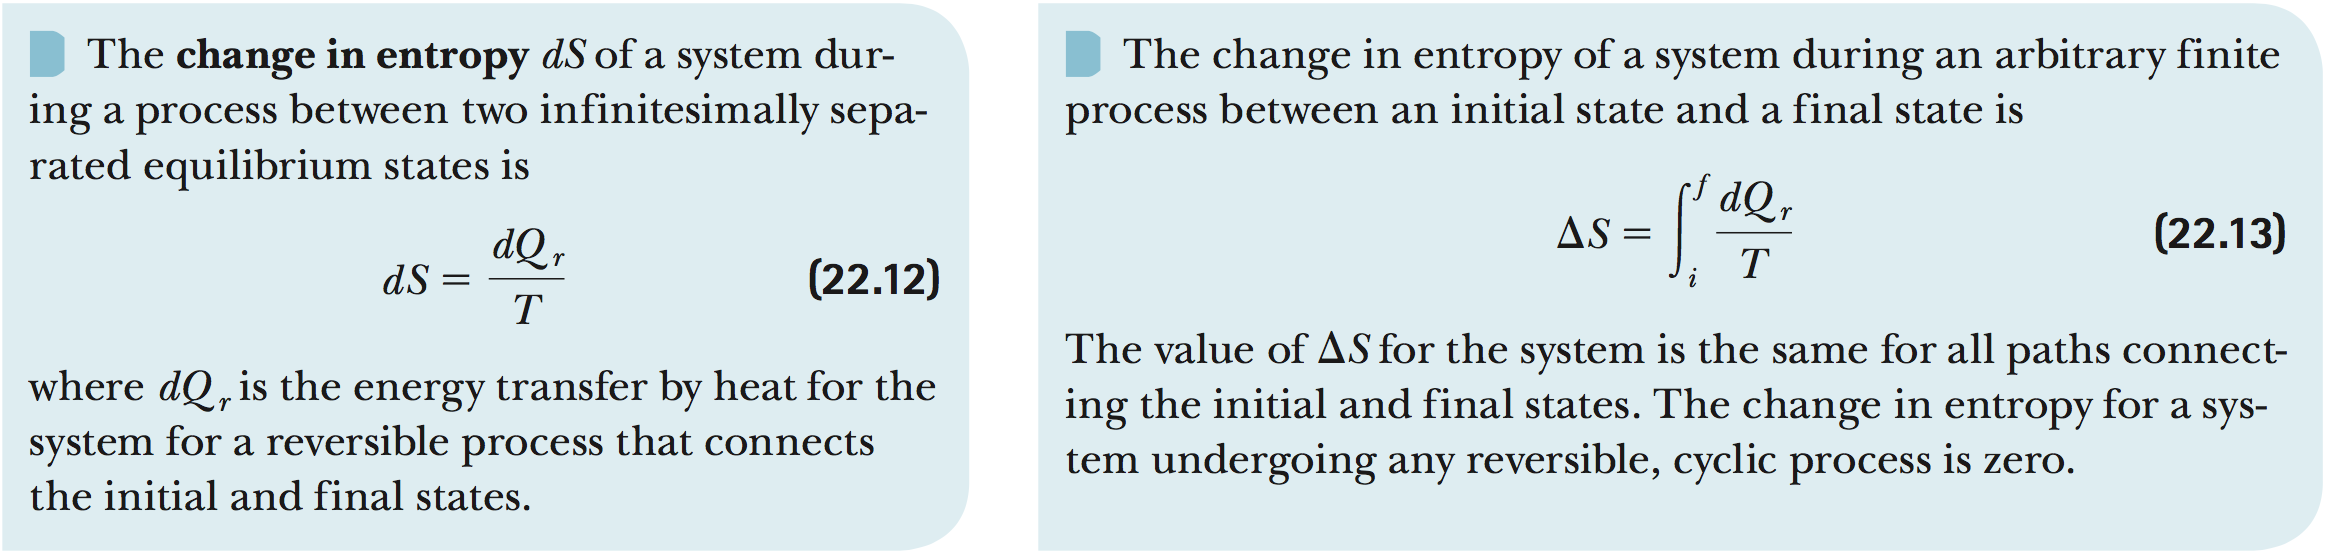
\includegraphics[scale=.42]{4_d.png}
	
\end{document}
